
\documentclass[a4paper,11pt]{article}

\usepackage{amsmath}
\usepackage{amssymb}
\usepackage{bm}
\usepackage{caption}
\usepackage{colortbl}
\usepackage{enumitem}
\usepackage{etaremune}
\usepackage{eurosym}
\usepackage{fancyhdr}
\usepackage{geometry}
\usepackage{graphicx}
\usepackage{lineno}
\usepackage{mathtools}
\usepackage{multicol}
\usepackage{multirow}
\usepackage{parskip}
\usepackage{setspace}
\usepackage{subcaption}
\usepackage{tabularx}
\usepackage{tabulary}
\usepackage{titlesec}
\usepackage[T1]{fontenc}
\usepackage{times}
\usepackage{url}
\usepackage{wrapfig}
\usepackage{xcolor}

\usepackage[colorinlistoftodos]{todonotes}

\usepackage{array}
\newcolumntype{C}[1]{>{\centering\arraybackslash}p{#1}}

% Shrink the spacing between references in the bibliography
%\usepackage{etoolbox}
%\patchcmd\thebibliography
% {\labelsep}
% {\labelsep\itemsep=-8pt\relax}
% {}
% {\typeout{Couldn't patch the command}}
 %%% End of code to add %%%

\bibliographystyle{h-physrev}

\renewcommand{\thesection}{\Alph{section}}

\newcounter{bar}
\newcommand{\taskcounter}{%
        \stepcounter{bar}%
        \thebar}

\setlist[itemize]{itemsep=-4pt, topsep=-2pt}

\usepackage{hyperref}

\hypersetup{ colorlinks=false,
		     linkcolor=green,
		     urlbordercolor=blue,
		     pdfborderstyle={/S/U/W 1}}
		     
\renewcommand{\smallskip} {\vspace{0.1in}}
\renewcommand{\medskip}   {\vspace{0.2in}}
\renewcommand{\bigskip}   {\vspace{0.4in}}

\geometry{tmargin=1.5cm, bmargin=1.5cm, lmargin=2cm, rmargin=2cm}

\setlength{\headheight}{15pt} 

\footskip=22pt
\headsep=18pt

\titlespacing*{\section}{0pt}{2pt}{2pt}
\titlespacing*{\subsection}{0pt}{2pt}{2pt}
\titlespacing*{\subsubsection}{0pt}{1pt}{1pt}


\singlespacing
%\linenumbers

%%%%%%%%%%%%%%%%%%%%%%%%%%%%%%%%%%%%%%%%%%%%%%%%%%%%%%%%%%
% Cover Page
%%%%%%%%%%%%%%%%%%%%%%%%%%%%%%%%%%%%%%%%%%%%%%%%%%%%%%%%%%

\begin{document}
\renewcommand{\headrulewidth}{0pt}

% \pagestyle{fancyplain}

% \lhead[\it Koskinen]{\it Koskinen}
% \chead{B1 - Cover Page}
% \rhead{NuUnity}

\vspace{1cm}

\centerline{ \large \textbf{ERC Starting Grant 2021}} \smallskip
\centerline{ \large \textbf {Research Proposal [Part B1]}} \smallskip

\vspace{1.0cm}

%
\centerline{\huge \textbf{A wrinkle in space-time}}
\vspace{0.5cm}
\centerline{ \huge {\bf (SpWrinkle)}} 


%~\\

\vspace{1.5cm}

\noindent
Cover page: \\
- Principal Investigator: Thomas Simon Stuttard\\
- Host Institution: Niels Bohr Institute (NBI), University of Copenhagen\\
- Proposal Duration: $60$ months\\

~\vspace{0. cm}

\noindent
{\bf Proposal Summary}:

The search for a quantum theory of gravity is one of the greatest open challenges in physics. The fluctuating nature of space-time expected in such a theory could produce observable impacts on neutrino propagation and oscillations, including neutrino decoherence, resulting in the damping of neutrino oscillations over distance, and CPT violation, manifesting as differing oscillation properties for neutrinos and antineutrinos.

I will perform the world’s most sensitive and comprehensive searches for these effects using a ground-breaking high statistics, high energy atmospheric neutrino data sample and pioneering neutrino-antineutrino separation techniques, using data from the upcoming upgrade to IceCube neutrino observatory at the South Pole. I will test a range of phenomenological models I have developed, including neutrino interactions with virtual black holes and lightcone fluctuations, achieving sensitivity to the naturally expected size of these effects for a Planck scale theory in a range of scenarios. In addition to testing quantum gravity, these results may even shed light on the Universe’s unexplained preference for matter over antimatter.


%%%%%%%%%%%%%%%%%%%%%%%%%%%%%%%%%%%%%%%%%%%%%%%%%%%%%%%%%%
% Extended Synopsis
%%%%%%%%%%%%%%%%%%%%%%%%%%%%%%%%%%%%%%%%%%%%%%%%%%%%%%%%%%
\newpage

\section{Extended Synopsis}
\vspace{0.1 cm}

\todo{Need less duplication in text from B2}
\todo{Need more technical details}

% \begin{wrapfigure}{R}{0.45\textwidth} %this figure will be at the right
%     \centering
% 		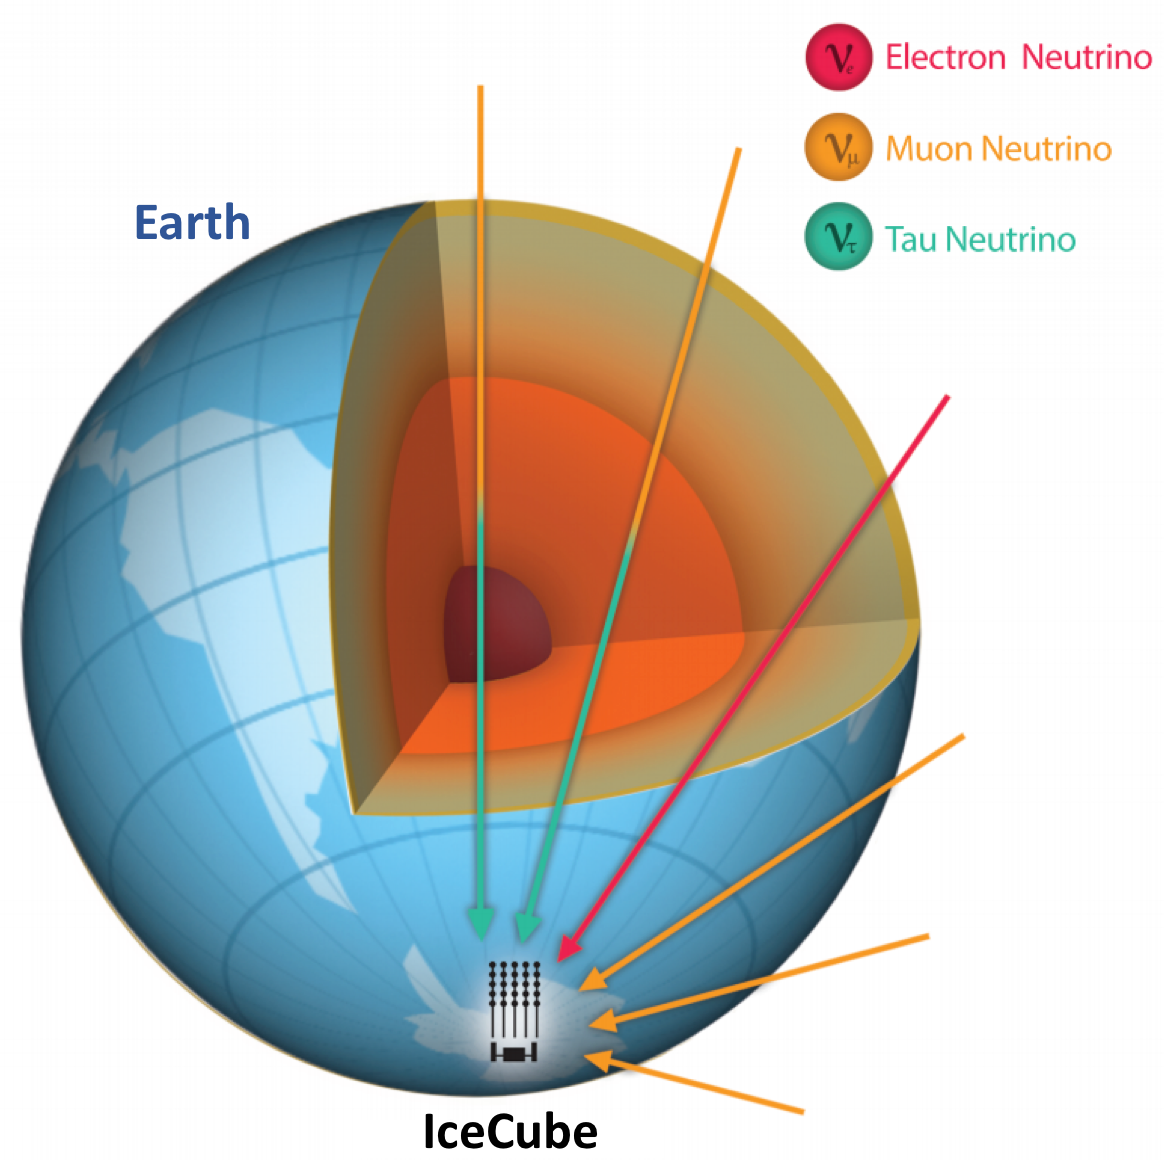
\includegraphics[width=1.\linewidth]{images/atmo_osc.png}
% 		\caption{Neutrinos produced in the atmosphere cross the Earth before detection in IceCube, oscillating and potentially experiencing the influence of quantum gravity as they propagate.}
% 		\vspace{-7pt}
% 		\label{fig:atmo_osc}
% \end{wrapfigure}

% \todo{Which figures?}
% \todo{Scan through B2 theory section and check if I'm missing any key points}

Despite every other force in Nature being successfully described by quantum mechanics and decades of theoretical efforts, there is currently no quantum theory of gravity. A major contributing factor to this impasse is the paucity of meaningful experimental constraints to guide theory, a consequence of the astounding weakness of gravity whose subatomic effects are expected to be suppressed\todo{discuss that SM is often considered to be a low energy something of a theory of everything} at the energy and distance scales we can experimentally probe, only becoming large at the \textit{Planck scale}; $10^{19}$\,GeV or $10^{-35}$\,m.

Although we do not have a complete quantum theory of gravity, we do know some of the features it is expected to exhibit, most notably that the fabric of space-time itself would be subject to the intrinsic uncertainty present in all quantum theories and fluctuate~\cite{PhysRev.97.511, Hawking}. This is predicted to result in \textit{lightcone fluctuations}~\cite{PauliLightcone, Ford1999, gr-qc/9909085, Ellis:1999jf}, where the fluctuating space-time curvature causes variations in the time taken by a particle to travel between two points, and the permeation of space with microscopic \textit{virtual black holes} (VBH)~\cite{Hawking1982,PhysRevD.53.3099}, continuously forming and evaporating in the gravitational analogue of the virtual electron-positron pairs of \textit{vacuum polarisation} in electromagnetism. 

Neutrinos offer one of the best opportunities to detect the weak effects of a quantum theory of gravity. They can travel vast distances unperturbed by other forces/matter, allowing the effects of quantum gravity at tiny distance scales to accumulate into potentially observable effects, and the bombardment of the Earth's atmosphere by cosmic rays produces a copious natural flux of neutrinos with energies exceeding even those produce at the LHC (up to PeV), allowing the suppression of quantum gravity effects to be at least partially overcome. 

\begin{wrapfigure}{R}{0.5\textwidth} %this figure will be at the right
    \centering
    \vspace{-7pt}
    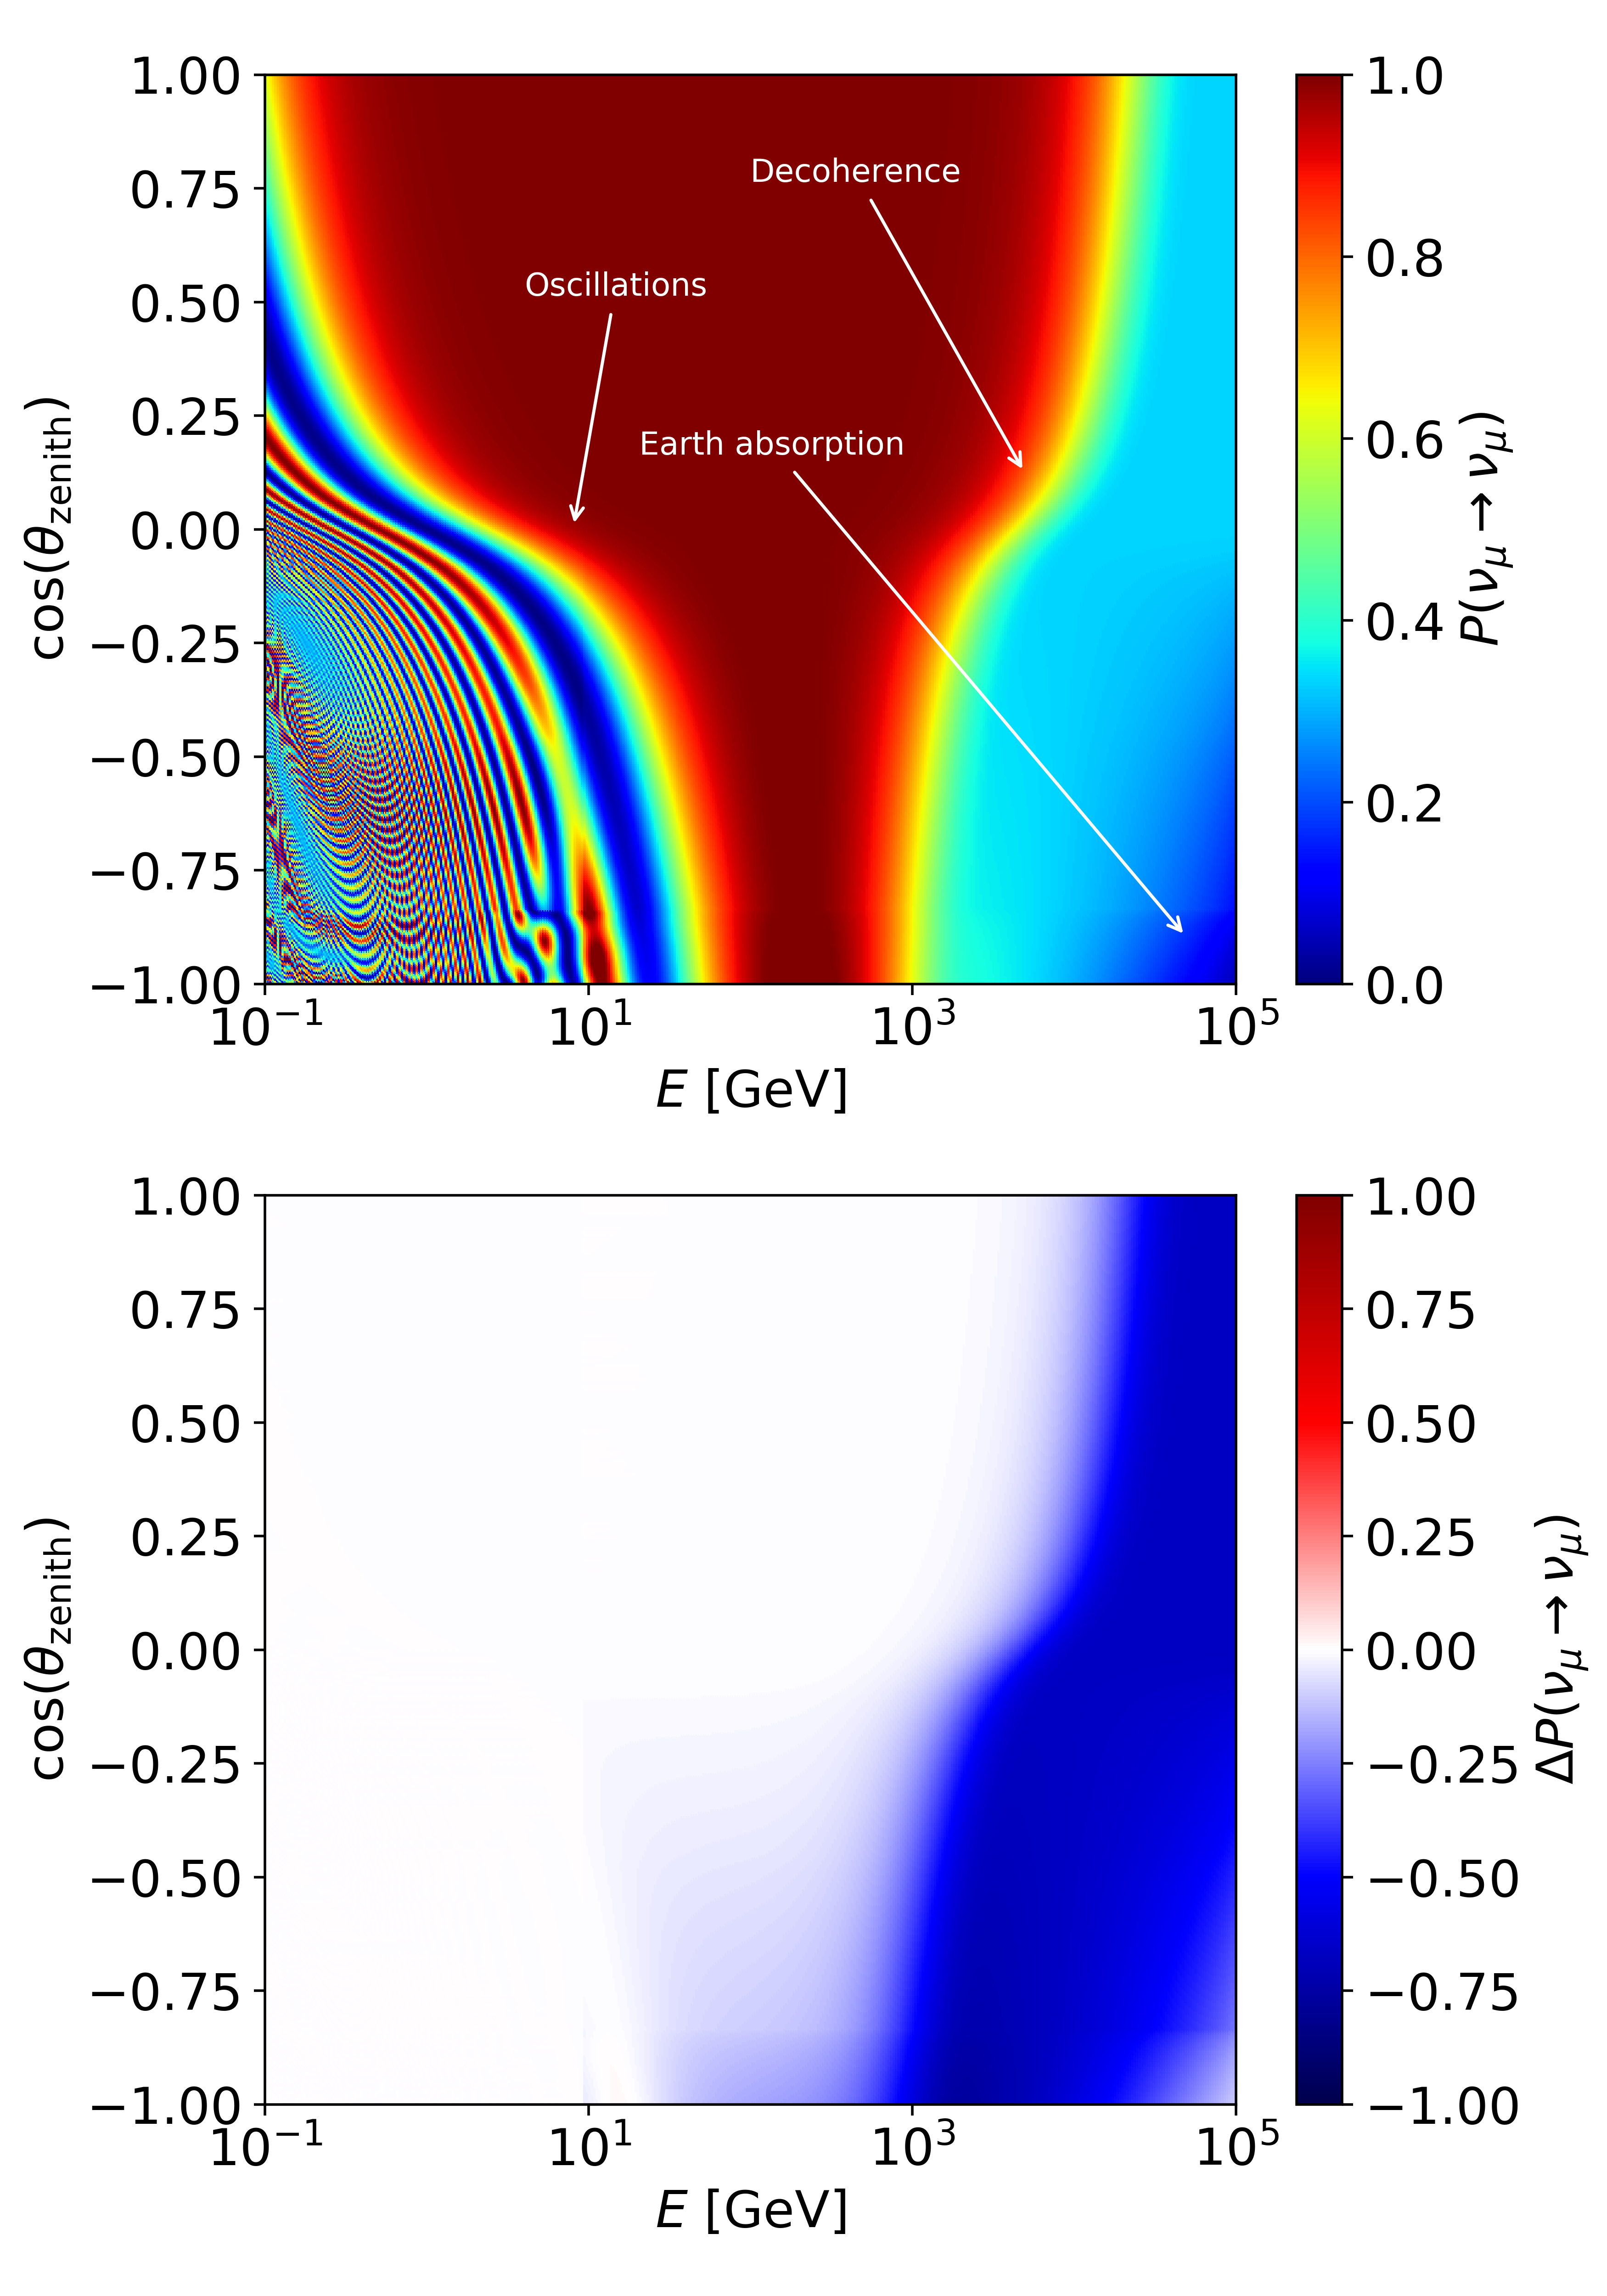
\includegraphics[trim=0.0cm 12.7cm 0.cm 0.2cm, clip=true, width=1.\linewidth]{images/atmo_oscillogram_randomize_flavor_n2_matter.png}
    \caption{Modified atmospheric neutrino oscillations vs. neutrino energy (x axis) and arrival direction (y axis) in one of my $\nu$-VBH interaction decoherence scenarios (with $E^2$ dependence)~\cite{PhysRevD.102.115003}.}
    \vspace{-5pt}
    \label{fig:decoh_oscillogram}
\end{wrapfigure}

The macroscopic quantum superposition effect of neutrino oscillations would be disrupted by these quantum gravity effects, providing an observable signal. Lightcone fluctuations would cause propagating neutrinos to become out phase with each over, resulting in neutrino decoherence and the damping of oscillations over distance. Interactions between propagating neutrinos and the stochastic VBH background would also produce decoherence effects (see Fig. \ref{fig:decoh_oscillogram}), with global symmetries potentially violated in such interactions~\cite{Anchordoqui:2005gj, Harlow:2018jwu, PhysRevD.102.115003, Hellmann:2021jyz}, resulting in flavour violations, conversions to different particle types or even the loss of the neutrino from the observable Universe altogether~\cite{Anchordoqui:2005gj, Anchordoqui:2006xv, Witten:2017hdv}. Even weak lightcone fluctuation and neutrino-VBH interaction effects can provide an observable signal in neutrino experiments which can collect extremely large statistics and span a large region of energy, such as the IceCube neutrino observatory, the world's largest neutrino detector with an active volume of 1 Gton.

Furthermore, a quantum theory of gravity violates a number of the prerequisites for $CPT$ symmetry, which only perfectly holds in flat space-time (clearly not the case at the scale of these space-time fluctations), and in unitary quantum theories where probability is conserved, whereas apparent unitarity violations could occur due to the loss of quantum information beyond the event horizons of the VBH background. The violation of $CPT$ symmetry ($CPT$-V) would result in differing properties (such as mass) between particles and antiparticles, with these differences suppressed below the Planck scale. Neutrino oscillations are sensitive to even sub-eV mass differences, making them a highly sensitive detection channel, with the signal being an asymmetry in the oscillations of neutrinos and antineutrinos. $CPT$-V searches also address one of the other major outstanding questions in particle physics; the origin of the matter-antimatter asymmetry of the Universe~\cite{Sakharov_1991}. Known differences between matter/antimatter (so-called $CP$-violations) can only account for a tiny fraction of the observed imbalance, meaning that new physics like $CPT$-V must exist, and the energy-suppressed effects tested here would have been strong in the high temperatures of the early Universe when (anti)matter was forming~\cite{Mavromatos:2017cxr, hep-ph/9809542, Ellis:2013gca}. \\

\subsection{Research objectives}

I will perform the world's most sensitive and comprehensive searches for energy-suppressed decoherence and $CPT$-V in neutrinos, including world first tests based on theoretical models I have developed, with the goal of detecting the first experimental signature of quantum gravity. To do so I will search for small modifications to neutrino propagation and oscillations using a state-of-the-art high statistics, high energy atmospheric neutrino data sample I will create using data from the IceCube neutrino observatory at the South Pole, as well as the next-generation IceCube Upgrade detector extension (to be completed in early 2024). I will also pioneer methods for separating neutrinos and antineutrinos for the first time in IceCube neutrino oscillation measurements, making the measurement of $CPT$-V oscillations possible and opening a new direction in new physics searches with IceCube. Crucially, I have demonstrated that these analyses are capable of detecting the predicted size of these quantum gravity effects in a number of scenarios, giving the realistic possibility of the first experimental detection of the signs of quantum gravity, a result that would be nothing short of revolutionary. 

I have developed models of neutrino decoherence resulting from neutrino-VBH ($\nu$-VBH) interactions~\cite{PhysRevD.102.115003} (including flavour violations, democratic population of particle states, severe phase perturbations and total loss of the neutrino) and lightcone fluctuations~\cite{2103.15313} (resulting from both fluctuating space-time curvature and intrinsic variability in the neutrino velocity, \textit{stochastic Lorentz invariance violation}~\cite{Vasileiou2015, Amelino-Camelia:2016fuh}) that I will test in this project. These models are the first to directly connect the observable phenomenology of neutrino decoherence to the underlying microphysics of a quantum theory of gravity, allowing experimental constraints on the fundamental nature of space-time to be made using decoherence measurements for the first time in this project. As the leader of the recent generation of world-leading IceCube neutrino oscillation measurements (with a team of 13 physicists from 7 institutes in Europe and the US) I have experience leading a major international research project, and play a leading role in the IceCube detector upgrade that this project will exploit. My scientific leadership skills have been recognised by the IceCube collaboration, where I hold the roles of \textit{IceCube Upgrade simulation manager} (I am the named responsible person to the US National Science Foundation for delivering all simulations for this \$37 million project) and \textit{IceCube oscillation physics co-convener}. My combined experimental, phenomenological and leadership expertise make me uniquely capable to lead my own independent research group to realise these ambitious and potentially revolutionary decoherence and $CPT$-V measurements, which are the result of my own scientific vision. \\

\todo{Statement about how this only happens if I get funded}

\todo{Do I actually say I am sensitive to Planck scale anywhere?}

\subsection{State-of-the-art}

In the absence of a concrete model of quantum gravity, it is essential to probe the broadest possible range of signals. Decoherence searches have been performed using neutrinos from nuclear reactors, the Sun, the Earth's atmosphere and particle accelerators~\cite{PhysRevLett.85.1166, Abbasi:2009nfa, PhysRevD.89.053002, Bakhti:2015dca, Coelho:2017zes, PhysRevD.95.113005, Coloma:2018idr, de_Holanda_2020}, although generally with simplified damping terms rather than specific models. The sensitivity of extragalactic neutrinos is limited despite their vast propagation distances by their unknown favour composition at source and incoherent nature of the observed diffuse flux~\cite{PhysRevD.102.115003}. The strongest constraints on energy-suppressed decoherence were set using low statistics publicly released IceCube atmospheric neutrino data~\cite{Coloma:2018idr}), which I will surpass by orders of magnitude in this project, as well as measuring new strongly energy-suppressed (cubic and quartic) scenarios that have not previously been experimentally tested, and will test an unprecedented range of models and with a robust treatment of systematic uncertainties not present in previous works, representing a major leap forward in this field.

Experimental constraints on $CPT$-V exist for neutral kaons~\cite{Ellis:1999xh, Ambrosino:2006ek, Abouzaid:2010ny, Babusci:2013gda, Schubert:2014ska}, neutrinos~\cite{Adamson:2013whj, Ohlsson:2014cha}, hadron colliders~\cite{Aad:2013eva, vanTilburg:2016awx} and in precision tests of low energy systems such as particle magnetic moment measurements~\cite{Bluhm:1997ci, Bennett:2007aa} and (anti)hydrogen spectroscopy~\cite{Kostelecky:2015nma}, with no observed signal to date. The most sensitive test of $CPT$-V neutrino oscillations to date comes from the MINOS neutrino accelerator experiment~\cite{Adamson:2013whj}, but under my leadership the precision of IceCube's neutrino oscillation measurements has reached parity with accelerator experiments for the first time and will surpass it with the data from the IceCube Upgrade. The precision measurements of neutrino oscillations that I will make, at orders of magnitude higher energies than accelerator experiments, will be significantly more sensitive to the energy-suppressed $CPT$-V effects expected in a quantum theory of gravity, and I will also explicitly test energy-dependent forms of $CPT$-V in high energy neutrino oscillations for the first time. Furthermore, tensions have emerged in neutrino vs antineutrino oscillation measurements~\cite{Abe:2019vii,NOvA_CP_result}, potentially indicating the presence of new physics that this project could reveal, making this measurement more important than ever. \\


% ------------------------------------------------------------------------------
% ------------------------------------------------------------------------------
% ------------------------------------------------------------------------------
% ------------------------------------------------------------------------------

\subsection{Methodology}
\vspace{0.1 cm}

The signals probed in this work manifest as second-order perturbations to known neutrino oscillation phenomena due to the energy-suppressed nature of quantum gravity effects. The IceCube neutrino observatory instruments 1 cubic kilometer of South Pole ice with 5160 photo-multiplier tubes (PMTs) to observe neutrino interactions of both atmospheric and astrophysical origin via Cherenkov light, and provides both the highest statistics and highest energy oscillating neutrino data sample in the world, making it the ideal instrument to search for these weak effects. The IceCube Upgrade project will in 2023-24 add 700 additional new multi-PMT optical modules, dramatically increasing detector efficiency and resolution in a dense 2 Mton core.

My team (one postdoc and two PhD students, with myself as PI) will use the first data from the upgraded IceCube detector to search for neutrino decoherence and $CPT$-V in neutrino oscillations, initially focusing on (a) modelling of the new IceCube Upgrade detector and (b) the challenging development of (anti)neutrino separation methods, before developing a huge neutrino data sample and testing it for the presence of these quantum gravity signals. A purchase of 10 GPUs will allow my team to develop simulation and machine learning methods efficiently (e.g. without competing for shared resources). \\



% \textbf{From instructions:} Describe the proposed methodology in detail including any key
% intermediate goals. Explain and justify the methodology in relation to the state of the art, and
% particularly novel or unconventional aspects addressing the 'high-risk/high-gain' balance. Highlight
% any intermediate stages where results may require adjustments to the project planning. 

% \todo{Do I need more info on IceCube in here?}


% The core deliverables of this project are the world's most sensitive (and in many cases first) searches for unique signatures of quantum gravity and the underlying nature of space-time, and for deviations between the properties of neutrinos and antineutrinos. In doing so and my team (one postdoc, two PhD students) and I are attempting to discover the first underlying indication of a unifying model of gravity at subatomic scales and an explanation for the overwhelming pervasiveness of matter rather than antimatter in the Universe. \\


\subsubsection{Neutrino-antineutrino separation}

\begin{figure}
%\begin{subfigure}[t]{0.5\textwidth}
    \begin{subfigure}[b]{0.5\textwidth}
    \centering
    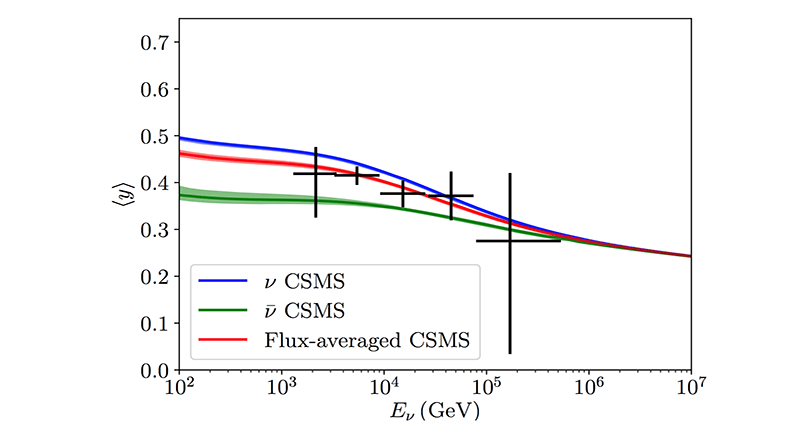
\includegraphics[trim=2.0cm 0.0cm 1.0cm 0.0cm, clip=true, width=\linewidth]{images/inelasticity.png}
    \caption{\label{fig:inelasticity}}
    \end{subfigure}
    \begin{subfigure}[b]{0.5\textwidth}
    \centering
    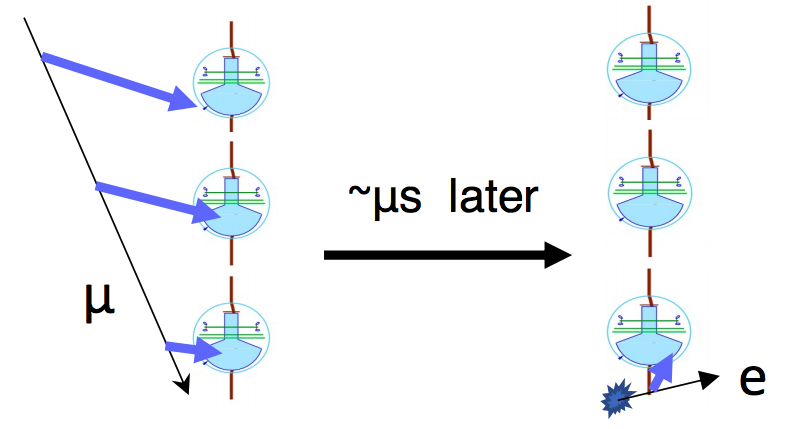
\includegraphics[trim=0.0cm 0.0cm 0.0cm 0.0cm, clip=true, width=\linewidth]{images/michel_electron.png}
    \caption{\label{fig:michel_electron}}
    \end{subfigure}
    \caption{(a) The average inelasticity, $\langle y \rangle$, of neutrino (blue) and antineutrino (green) interactions in IceCube, which differs in the energy range probed in this work~\cite{Aartsen:2018vez}. (b) A muon ($\mu$) from a neutrino interaction deposits light in the detector (leading to a reconstructable track) before stopping. Microseconds later the stopped muon decays, producing a Michel electron ($e$) which itself produces detectable light in the nearest sensor.}
    \vspace{-7pt}
\end{figure}

The most challenging but highest impact technical aspect of this project is the development of the first neutrino-antineutrino discrimination techniques to be used in neutrino oscillation measurements in IceCube, enabling fpr the first time the pioneering high energy $CPT$-V measurements I will make, and is prioritised early in the schedule to allow re-allocation of additional resources should delays occur. The properties of the neutrino interactions observed by IceCube that can separate (anti)neutrinos are are:

\begin{itemize}[leftmargin=*]
    \item The interaction \textit{inelasticity} (fraction of the incoming neutrino energy transferred to the ice nucleus) is on average $\sim$10-50\%  higher for neutrinos than antineutrinos in the energy range of interest (see Fig. \ref{fig:inelasticity}). Inelasticity reconstruction for muons has been achieved for TeV neutrinos~\cite{Aartsen:2018vez}, and I have demonstrated that the IceCube Upgrade will enable inelasticity reconstruction with $\sim$10\% resolution for even GeV events.
    \item The (anti)muons produced in muon (anti)neutrino interactions eventually come to rest and decay in the ice, producing a \textit{Michel electron} that yields delayed light a few microseconds later ($\sim$5000 photons per decay). The decay lifetime differs for (anti)muons due to capture of muons on oxygen nuclei in the ice, meaning that the time of this delayed light can distinguish between neutrinos vs. antineutrinos (Fig. \ref{fig:michel_electron}). My oscillation physics working group has demonstrated the feasibility of detecting the delayed light from Michel electrons, showing that such light is detected in $\sim$5\% of IceCube events.
\end{itemize}

I will build on these initial studies to pioneer the first use of (anti)neutrino separation in IceCube neutrino oscillation measurements, reconstructing inelasticity by simultaneously reconstructing the energy of the cascade-like light emission from the break up of the ice nucleus and track-like secondary muon emission in charged-current muon neutrino interactions ($\sim$80\% of events), and using the precise muon track reconstruction afforded by the IceCube Upgrade sensors to pinpoint the muon decay vertex and tag delayed light in the nearby optical sensors. I will combine both these inputs in a machine learning classifier to separate neutrinos from antineutrinos on a statistical basis, and exploit the vast flux of muons from cosmic ray air showers detected by IceCube ($\sim$100 billion per year) to perform data-driven verification of the muon decay vertex and delayed light tagging methods that can be compared to signal simulations.

% This a central and highly challenging element of this project, requiring the development and integration of multiple brand new experimental methods. However, a successful (anti)neutrino classifier will be truly game-changing for IceCube oscillation physics, paving the way for new physics searches with differing (anti)neutrino signals including Non-Standard Interactions with complex couplings, sterile neutrinos and the determination of the neutrino mass ordering, not to mention the $CPT$-V searches in this project. These methods can also be used to probe the antineutrino content of the astrophysical neutrino flux observed by IceCube~\cite{Aartsen:2013jdh}, constraining their production mechanisms (a major open question in neutrino astronomy)~\cite{glashow_icecube} \todo{this paragraph needs more specifics}.

\todo{Focus more on impact for my measuremnt}

\textbf{Deliverables:} Inelasticity reconstruction and delayed light tagging methods, (anti)neutrino classifier. \\

\subsubsection{Simulations}

% \begin{wrapfigure}{R}{0.35\textwidth} %this figure will be at the right
%     \centering
%     % \vspace{-7pt}
%     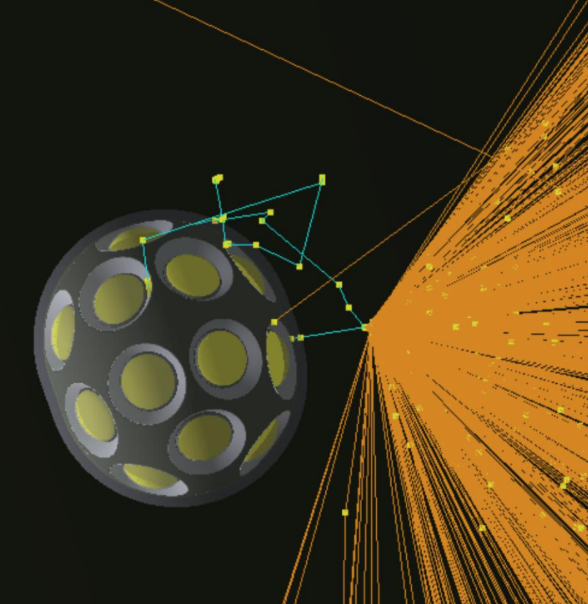
\includegraphics[trim=0.0cm 0.0cm 0.cm 1.0cm, clip=true, width=\linewidth]{images/mDOM_noise.png}
%     % \end{subfigure}
%     \caption{Visualisation of a prototype GEANT4 simulation of one of the new optical sensors in the IceCube Upgrade. A radioactive decay event is shown.}
%     % \vspace{-7pt}
%     \label{fig:mDOM_sim}
% \end{wrapfigure}

In these measurements I will quantity the impact of neutrino decoherence and $CPT$-V in IceCube via the comparison of simulated signals to the observed detector data. I will develop high fidelity data-driven simulation models of the new IceCube Upgrade optical sensors, most crucially the after-pulsing in the PMTs (up to microseconds after genuine signal hits), and sensor noise resulting from the radioactive decays of impurities in the glass surrounding the optical modules, both of which can mimic the Michel electron signal that is fundamental to (anti)neutrino separation. The noise rates are $>10 \times$ larger in these new modules than existing IceCube sensors, and will feature a correlated component across the multiple PMTs in a single sensor (resulting from Cherekov light from electrons in the radioactive decay chains), with the chance coincidence of light from multiple decays will be the dominant source of background for neutrino interactions in the IceCube Upgrade. Accurate characterisation of the time and charge distributions of these after-pulse and noise backgrounds is essential to quantify the \textit{false positive} rate in the delayed light tagging and any irreducible noise backgrounds in the neutrino sample, to avoid bias (and potentially a spurious signal) in the decoherence and $CPT$-V measurements. These models will be benchmarked against laboratory test data taken concurrently by my collaborators at Michigan State University, M{\"u}nster University and DESY-Zeuthen, and the model development is prioritised at the start of the project to allow iteration on these test procedures should unexpected behaviour be identified.

% The measurement principal to be used in this project is the comparison of simulated new physics signals and resulting detector response to observed data. I will develop software models of the new segmented optical sensors to be deployed in the IceCube Upgrade, including their geometry, photo-multiplication stage, readout electronics and noise (from the radioactive decays of impurities in the glass sensor housing), replacing the simple and imprecise parameterisations currently used in IceCube simulations with `industry standard' \texttt{GEANT4}~\cite{Agostinelli:2002hh} models. I will verify and tune these models against laboratory test data and ultimately using the first data from the deployed detector, with my team travelling to the South Pole to assist the detector installation and utilise these simulations to verify the operation of the deployed hardware in real-time \todo{Alongside lab tests}.

% \todo{More on why this is important, e.g. biases and spurious nu nubar signals especially}

I will then combine these models with existing event generator and photon propagation software to produce high statistics Monte Carlo (MC) simulation samples of both neutrino interactions and background events (atmospheric muons and coincident detector noise) in IceCube for comparison to detector detector when evaluating the decoherence/$CPT$-V signals. I am collaborating with the developers of a high energy extension~\cite{Garcia:2019hze} to the state-of-the-art \textit{GENIE} neutrino interaction generator~\cite{Andreopoulos:2009zz} to develop consistent modeling of neutrino interactions across the full GeV to PeV energy range probed in these analyses for the first, requiring updates to the parton distribution functions (PDFs) used for $<$100 GeV interactions (with interpolation between the existing models being a fall back option is these updates cannot be completed in time for these measurements), and will integrate cross section tuning data provided by accelerator neutrino experiments. 

Under my leadership as \textit{IceCube Upgrade simulation manager}, my collaborators and I have developed initial prototypes of these simulations, which were fundamental to demonstrating the physics potential of the IceCube Upgrade and its successful funding. This, combined with my experience in high fidelity detector modelling from my Ph.D. -- where I developed simulations of the tracking tracking detector the Fermilab muon g-2 experiment, which were a fundamental component of the most precise high energy particle physics measurement in history~\cite{gm2_run1_result} -- and four years of experience as a professional simulations engineer in the space industry before my academic career (developing simulations of the European Space Agency's ExoMars Rover, Solar Orbiter and GAIA missions), makes me ideally suited to this task. 

\textbf{Deliverables:} Optical sensor models (geometry, quantum efficiency, amplification, after-pulsing, noise, readout electronics). MC simulation samples (with 10$\times$ detector data statistics) of neutrino interactions, atmospheric muons and coincident noise in the detector. \\


\subsubsection{Event sample}

At the core of these measurements will be the first atmospheric neutrino data sample spanning the full energy reach of IceCube (GeV to PeV), containing well over 1 million neutrinos to provide unprecedented statistics for neutrino physics, allowing these measurements to probe both the GeV region where oscillations are strongest and TeV/PeV high energy regime where quantum gravity signals may be magnified. I will unify disparate background rejection (removing $\mathcal{O}(10^6)$ atmospheric muon and coincident noise background events for every neutrino) and neutrino energy/direction/flavour reconstruction methods from the GeV and TeV regimes, in particular using TeV+ cascade-like events in an IceCube oscillation measurement for the first time to give sensitivity to high energy anomalous muon to tau neutrino oscillations which are the dominant expected signal. I will exploit the segmented and densely packed nature of the new sensors to veto the punishing rate of noise background triggers in the IceCube Upgrade by identifying events with light signatures causally inconsistent with a common source, building upon my experience developing the most powerful noise rejection methods in IceCube to date (the first applications of machine learning to this task).

Fully exploiting the new multi-PMT optical modules requires developments of entirely new neutrino reconstruction techniques, and the development of deep learning neural network reconstruction methods suited to the irregular IceCube detector geometry (e.g. not tied to the regular pixel structure assumed by standard image processing techniques) is well underway within the IceCube collaboration, with a prototype graph neutral network (GNN) based method developed in a  collaboration between machine learning experts from the ATLAS experiment and myself already showing $\sim$30\% improvement in resolution over the current state-of-the-art methods in IceCube and is naturally extendable to the IceCube Upgrade. 

\textbf{Deliverables:} Neutrino data sample with over 1 million GeV-PeV neutrinos with reconstructed energy, direction, flavour and (anti)neutrino classification, with $\sim$1\% background contamination. \\

\subsubsection{Systematic uncertainties}

The large statistical power of these measurements and weakness of the sought-after signals demand a robust treatment of systematic uncertainties to avoid biases. I will characterise the impact of detector calibration uncertainties on the analyses, including the PMT quantum efficiency, noise rates and position/orientation of the new optical sensors -- which are deployed down 2 km long cables into melted and subsequently re-frozen holes in the ice -- and the optical properties of these re-frozen ice columns, by re-simulating neutrino interactions in the detector with the optical sensor model input parameters varied within the calibrated uncertainty range, and parameterise the resulting changes to reconstructed neutrino properties for use a nuisance parameters in the decoherence/$CPT$-V measurements. 

The composition of the atmospheric neutrino flux is another major source of systematic uncertainty due to uncertainties in the spectrum of cosmic rays reaching the Earth, atmospheric conditions, and the modelling of hadronic processes governing the air shower development, and these flux uncertainties can mimic the energy-dependent signals under test. I will exploit the copious flux of atmospheric muons detected by IceCube to develop a high statistics muon `sideband' and simultaneously fit this alongside the neutrino data during these measurements, both strongly constraining the air shower uncertainties and acting as a control sample for evaluating the modelling of the detector independently of the neutrino physics signals. This will be the first use of this novel method in IceCube. 

%There is synergy here with ongoing activities at NBI, where a muon sample is being developed for calibration of the quantum efficiency of the PMTs which can serve as a starting point for this sideband to accelerate its development.  \\

\textbf{Deliverables:} Models of the impact of optical module calibration systematic uncertainties on neutrino data sample, integrated into analysis framework as nuisance parameters. Atmospheric muon sideband data sample, incorporated into analysis pipeline with integrated muon and neutrino air shower flux systematic uncertainty modelling.  \\

% \subsubsection{Signal modelling}

% \todo{Move this into analusis section}

% \todo{Some of this to B2?}

% I will model the influence of the new physics probed in this work on neutrino propagation using the state-of-the-art \texttt{nuSQuIDS} quantum state evolution software~\cite{Delgado:2014kpa, nusquidsGIT} and including an accurate treatment of the interplay between these signals and standard matter in the Earth on neutrino propagation. Both decoherence and $CPT$-V have been predicted from varied new physics scenarios, meaning these measurements are potentially sensitive to the properties of string theories~\cite{Mavromatos2010, AmelinoCamelia:2008qg} (including the holographic principal~\cite{Perlman_2015, Harlow:2018jwu}), black hole information theory~\cite{PhysRevD.102.115003, Hellmann:2021jyz}, new particles~\cite{Hellmann:2021jyz}, neutrino interactions with Dark Matter~\cite{1909.11271, EPJC802020, Capozzi:2018bps, 1904.02518} and the diffuse gravitational wave background~\cite{PhysRevD.100.096014}. To this end I will host a specialised workshop on neutrino decoherence and $CPT$-V to further develop these scenarios with a view to testing additional models in this project.

% \textbf{Deliverables:} \textit{nuSQuIDS} implementations of lightcone fluctuation, $\nu$-VBH and $CPT$-V models (plus additional models identified during phenomenological work), integrated into analysis framework.  \\

\subsubsection{$CPT$-V and decoherence data analysis}

The event sample and simulations developed in this project will form the core of both the $CPT$-V and decoherence analyses, which will search for distortions in the atmospheric neutrino spectrum in IceCube in 4-dimensions; reconstructed neutrino energy, arrival direction (a proxy for travel distance), flavour, and neutrino vs antineutrino. I will model the influence of the new physics probed in this work on neutrino propagation using the state-of-the-art \texttt{nuSQuIDS} quantum state evolution software~\cite{Delgado:2014kpa, nusquidsGIT} (including a full treatment of the interplay between these signals and standard matter effects on neutrino propagation in the Earth), and will host a workshop on neutrino quantum gravity phenomenology to develop further decoherence/$CPT$-V scenarios that can be tested in these measurements, drawing upon the \textit{COST Action CA18108 (quantum gravity phenomenology)} network of which I am an active member. 

% Both decoherence and $CPT$-V have been predicted from varied new physics scenarios, meaning these measurements are potentially sensitive to the properties of string theories~\cite{Mavromatos2010, AmelinoCamelia:2008qg} (including the holographic principal~\cite{Perlman_2015, Harlow:2018jwu}), black hole information theory~\cite{PhysRevD.102.115003, Hellmann:2021jyz}, new particles~\cite{Hellmann:2021jyz}, neutrino interactions with Dark Matter~\cite{1909.11271, EPJC802020, Capozzi:2018bps, 1904.02518} and the diffuse gravitational wave background~\cite{PhysRevD.100.096014}. To this end I will host a specialised workshop on neutrino decoherence and $CPT$-V to further develop these scenarios with a view to testing additional models in this project.

For the $CPT$-V search I will separately fit the oscillation properties of neutrinos and antineutrinos, in particular performing the world's first test of energy-dependent deviations, motivated by the expectation that the effects of quantum gravity are suppressed below the Planck scale. Variations in mixing angle produce effects at GeV scales where conventional oscillation effects are strong, whilst differing (anti)neutrino masses can resulting in anomalous oscillations across the full energy range of the analysis.

% \textbf{Risk/Gain:} The $CPT$-V measurement is made possible by the pioneering but extremely challenging (anti)neutrino separation techniques developed in this project, giving an unparallel opportunity to test energy-suppressed $CPT$-V scenarios to which accelerator experiments are blind. This work is prioritised early in the project so that additional resources can be re-allocated to it if required.

The signal of neutrino decoherence in IceCube is the (energy-dependent) damping of neutrino oscillations over distance, maximal for neutrinos cross the Earth's full diameter ($\sim$12,700 km). I will perform both a generalised decoherence search (fitting matrix elements of a decoherence operator modelling the neutrino and its environment as an \textit{open quantum system}~\cite{lindblad1976, Benatti_2000, gago2002study, PhysRevLett.85.1166} and tests of my $\nu$-VBH interaction and lightcone fluctuation models, fitting the underlying model parameters. $CPT$-V is also predicted to manifest as differences between neutrino and antineutrino decoherence effects~\cite{Mavromatos_2009, Barenboim:2004wu, Carrasco:2018sca, Buoninfante:2020iyr, Capolupo:2020myw}, and I will exploit this opportune synergy in this project to also perform the world's first search for $CPT$-V decoherence, giving the prospect of detecting $CPT$-V even if neutrino-antineutrino mixing angle and mass differences prove immeasurably small. 

% Crucially this analysis will achieve sensitivity to the naturally expected scale of quantum gravity effects for the $\nu$-VBH interactions models tested up to even cubic energy-suppression, guaranteeing either the first detection of quantum gravity or the rejection of a range of well motivated models. Either way these results will be invaluable in informing the theoretical development of quantum gravity. I will also perform a model-independent search (the first of its kind), fitting the matrix elements of a generalised \textit{decoherence operator}, expressed in the mathematical framework of , giving sensitivity to virtually any possible source of neutrino decoherence. 

% \textbf{Risk/Gain:} The development of an event sample spanning six orders of magnitude in energy is a major challenge, but will yield unprecedented sensitivity to the broadest range of decoherence scenarios ever tested.

% \textbf{Risk/Gain:} This generalised decoherence search will feature many free parameters in the fit, a major computational challenge for the frequentist \textit{minimisation} algorithms used in most oscillation analyses. Should this prove untenable, I will instead employ Bayesian Markov Chain Monte Carlo (MCMC) methods which have been shown to perform better in many parameter fits. This will require a significant time investment implementing these methods in my analysis software framework\todo{Probably drop this - boring}.

\textbf{Deliverables:} Model-independent measurement of energy-dependent coherence length of neutrinos, world first measurements of the $\nu$-VBH interaction mean free path, neutrino propagation distance fluctuations, neutrino stochastic Lorentz invariance violation, and $CPT$-V decoherence operators. Measurements of energy-dependent deviations between (anti)neutrino atmospheric mixing angle ($\theta_{23}$) and mass splitting ($\Delta m^2_{32}$).

\textbf{Impact:} \todo{TODO. Planck scale limit} \\

\subsubsection{Conclusions}

% TODO See Jason's \\

\todo{Neutrinos are o e of the best morivated serch channels in what must necessarily be an extrmely varied global quantum qravity searc progra. The searches of indication of anaomolous oscillations in high enery neutrinos... }

This project will produce genuinely game changing advances in both experimental searches for quantum gravity with neutrinos and in the technical sophistication of IceCube data analysis methods, achieving rare sensitivity to Planck scale physics. \\


% ------------------------------------------------------------------------------
% ------------------------------------------------------------------------------
% ------------------------------------------------------------------------------

%\begin{multicols}{2}
\bibliography{references}
%\end{multicols}


%%%%%%%%%%%%%%%%%%%%%%%%%%%%%%%%%%%%%%%%%%%%%%%%%%%%%%%%%%
% CV
%%%%%%%%%%%%%%%%%%%%%%%%%%%%%%%%%%%%%%%%%%%%%%%%%%%%%%%%%%
\newpage

\section{Curriculum Vitae}

% \chead{B1 - Curriculum Vitae}

\vspace{0.2cm}
\textbf{PERSONAL INFORMATION ~~\hrulefill}\smallskip\\
Name: Thomas Simon Stuttard \\
Date of Birth: 3rd December 1985\\
Nationality: British

%=======================================================================
%=======================================================================
% Education
%
\vspace{0.2cm}
\textbf{EDUCATION ~~\hrulefill}\smallskip\\
%
{\bf PhD in Physics} \hfill {\em 2017} \\ 
University College London, United Kingdom // Fermilab muon g-2 experiment

{\bf MSci in Physics and Astrophysics, 1st class} \hfill {\em 2009} \\ 
University of Bristol, United Kingdom \\
Awarded the Masters thesis prize (International Linear Collider, ILC)

% \begin{tabular*}{\textwidth}%
%   {@{\extracolsep{\fill}}lcr}
%   2017 & PhD in Physics \\
%   & University College London, UK \\
%   & Supervisor: Professor Mark Lancaster \\
%   %\multicolumn{3}{l}{- Advisor: Prof. Jenny Thomas} \smallskip
%   \\
%   University of Minnesota-Duluth & \bf{M.S.}, Physics & 2004 \\
%   %\multicolumn{3}{l}{- Advisor: Prof. Alec Habig} \smallskip
%   \\ 
%   Rensselaer Polytechnic Institute & \bf{B.S.}, Physics & 2002 \\
% \end{tabular*}
% ~\smallskip \\
% \indent
%
%== End Education block
%
%=======================================================================
%=======================================================================
\vspace{0.2cm}
\textbf{CURRENT POSITION ~~\hrulefill}\smallskip\\
%
{\bf Assistant professor} \hfill {\em 2020 - present} \\ 
Niels Bohr Institute, Denmark // IceCube

\vspace{0.2cm}
\textbf{PREVIOUS POSITIONS ~~\hrulefill}\smallskip\\
%
{\bf Postdoc} \hfill {\em 2016 - 2020} \\ 
Niels Bohr Institute, Denmark // IceCube

{\bf Simulation Engineer} \hfill {\em 2009 - 2013} \\ 
Airbus Space (formerly EADS Astrium), United Kingdom \& France\\
European Space Agency ExoMars Rover, Solar Orbiter and GAIA missions. \\
Project leader of Solar Orbiter platform and payload simulations (6 engineers across 3 countries). \\
This industry position was prior to my PhD and the start of my academic career. 

%=======================================================================
%=======================================================================
\vspace{0.2cm}
\textbf{SUPERVISION OF GRADUATE STUDENTS AND POSTDOCTORAL FELLOWS ~~\hrulefill}\smallskip\\
%
{\bf MSc} \hfill {\em 2017 - present} \\
5 students (co-supervisor), Niels Bohr Institute, Denmark
% Kasper Pedersen (ongoing), Jonathan Jegstrup (ongoing), Thomas Halberg (2019), Ida Storehaug (2019), Mikkel Jensen (2089)

%=======================================================================
%=======================================================================
\vspace{0.2cm}
\textbf{ORGANISATION OF SCIENTIFIC MEETINGS ~~\hrulefill}\smallskip\\
%
{\bf International PhD Summer School on Neutrinos} \hfill {\em 2021} \\ 
  Niels Bohr Institute, Denmark - Co-organiser
  
{\bf Particle Physics with Neutrino Telescopes (PPNT)} \hfill {\em 2019} \\ 
  Uppsala University, Sweden (39 participants) - Session chair
  
{\bf IceCube Upgrade design workshop} \hfill {\em 2019} \\ 
  Michigan State University, US (35 participants) - Session organiser

{\bf IceCube Upgrade simulation and reconstruction workshop} \hfill {\em 2018} \\ 
  Niels Bohr Institute, Denmark (19 participants) - Primary workshop organiser

{\bf IceCube oscillation analysis software code sprint} \hfill {\em 2018} \\ 
  Niels Bohr Institute, Denmark (5 participants) - Primary workshop organiser

{\bf Niels Bohr Institute experimental neutrino physics journal club} \hfill {\em 2017 - present} \\ 
Primary organiser of bi-weekly event with $\sim20$ attendees, bridging gap between theorists and experimentalists.

% \todo{Collab meeting, osc meetings}
  
%=======================================================================
%=======================================================================
\vspace{0.2cm}
\textbf{INSTITUTIONAL AND RESEARCH RESPONSIBILITIES ~~\hrulefill}\smallskip\\
%
{\bf IceCube neutrino oscillation physics working group co-convener} \hfill {\em 2018 - present} \\ 
Leading oscillations working group in IceCube ($\sim$30 scientists in 11 institutes - US, Canada, Germany, UK and Denmark), including Beyond Standard Model (BSM) oscillations. Responsible for all oscillation analyses and publications, weekly conference calls and twice-annual collaboration meetings in Europe, US and Japan. 

{\bf IceCube Upgrade Simulation Manager} \hfill {\em 2018 - present} \\ 
Managing collaboration-wide simulation efforts for the IceCube Upgrade. Named responsible person to the US National Science Foundation for the simulation of all in ice detector and calibration devices. Also coordinating reconstruction, data processing and analysis efforts during the detector development phase.

{\bf IceCube Upgrade Technology Board} \hfill {\em 2018 - present} \\ 
Member of board overseeing technology requirements, development, procurement, quality control and commissioning for the IceCube Upgrade.

{\bf IceCube Coordination Committee} \hfill {\em 2018 - present} \\ 
Member of committee coordinating IceCube human and computing resources, software priorities, and connections between technical and science working groups.

{\bf European Committee for Future Accelerators (ECFA) } \hfill {\em 2019} \\ 
Early career scientist representative for Denmark.

{\bf Snowmass 2021 } \hfill {\em 2020 - present} \\ 
IceCube point of contact for neutrino oscillation physics for US Particle Physics Community Planning. \\
Primary author of all IceCube neutrino oscillation contributions to Snowmass 2021.

{\bf COST Action CA18108 quantum gravity phenomenology reviewer  } \hfill {\em 2021} \\ 
Invited contributor to pan-European review, primary author for topic of neutrino decoherence.

%=======================================================================
%=======================================================================
\vspace{0.2cm}
\textbf{MAJOR COLLABORATIONS ~~\hrulefill}\smallskip\\
%
{\bf IceCube collaboration} \\ 
Member of the 300-person IceCube collaboration across Europe, US and Asia.

{\bf COST Action CA18108: Quantum gravity phenomenology in the multi-messenger approach} \\ 
Member of an international collaboration seeking evidence of quantum gravity.

{\bf Fermilab muon g-2 collaboration} \\ 
Member of the 200-person international collaboration searching for new physics with precision muon measurements.


%
%%%%%%%%%%%%%%%%%%%%%%%%%%%%%%%%%%%%%%%%%%%%%%%%%%%%%%%%%%
% Funding ID
%%%%%%%%%%%%%%%%%%%%%%%%%%%%%%%%%%%%%%%%%%%%%%%%%%%%%%%%%%
\newpage 

\lhead[\it Koskinen]{\it Koskinen}
\chead{B1 - Funding ID}
\rhead{NuUnity}


%~\vspace{2cm}

\centerline{ {\textit{\textbf{ Appendix: All on-going and submitted grants and funding of the PI (Funding ID)}}
}} \smallskip
\centerline{ \it \underline{Mandatory information} (does not count towards page limits)
}\smallskip

~\vspace{2cm}

{\bf Current grants}
\begin{table}[h]
\centering
\begin{tabularx}{1\textwidth}{|C{0.125\textwidth}|C{0.125\textwidth}|C{0.1\textwidth}|C{0.115\textwidth}|C{0.115\textwidth}|C{0.26\textwidth}|}
\hline
\rowcolor[gray]{0.85} \it Project~Title & \it Funding Source & \it Amount (Euros) & \it Period & \it Role of the PI & \it Relation to current ERC Proposal\\
\hline
None  & & & & & \\
\hline
\end{tabularx}
\end{table}

~\vspace{2cm}


{\bf On-going and submitted grant applications}
\begin{table}[h]
\centering
\begin{tabularx}{1\textwidth}{|C{0.125\textwidth}|C{0.125\textwidth}|C{0.1\textwidth}|C{0.115\textwidth}|C{0.115\textwidth}|C{0.26\textwidth}|}
\hline
\rowcolor[gray]{0.85} \it  Project Title & \it Funding Source & \it Amount (Euros) & \it Period & \it Role of the PI & \it Relation to current ERC Proposal\\
\hline
DFF Project 1 & Independent Research Fund Denmark & 387,159.04 & Jan 2022 -- Dec 2024 & Principal Investigator & A more limited neutrino decoherence analysis using the first year of IceCube Upgrade data. \\
\hline
DFF Sapere Aude & Independent Research Fund Denmark & 832,512.20 & Aug 2022 -- Mar 2026 & Principal Investigator & Also aims to perform neutrino decoherence and $CPT$-V analyses with IceCube Upgrade data, but with a more limited scope. \\
\hline
\end{tabularx}
\end{table}

%%%%%%%%%%%%%%%%%%%%%%%%%%%%%%%%%%%%%%%%%%%%%%%%%%%%%%%%%%
% Track Record
%%%%%%%%%%%%%%%%%%%%%%%%%%%%%%%%%%%%%%%%%%%%%%%%%%%%%%%%%%

\newpage

\subsection{Track record}

\vspace{0.2cm}

% \textbf{From instructions:} Section c: Early achievements track-record (max. 2 pages) should list your important achievements,
% including your most important publications27 (up to five for Starting Grant and up to ten for
% Consolidator Grant) highlighting those as main author and/or without the co-authorship of your PhD
% supervisor. The publications should be properly referenced, including all authors in the published
% order (Please see section 1.1 on Research integrity). Field relevant bibliometric indicators as well as
% research monographs and any translations thereof may also be included. If applicable include:
% granted patent(s); invited presentations to internationally established conferences and/or
% international advanced schools; Prizes/Awards/Academy memberships etc. 

\textbf{Bibliometric indicator:} h-index = 22 (peer-reviewed publications only, calculated using \texttt{inspire-hep}) \\
\textbf{ORCID:} 0000-0001-7944-279X

\vspace{0.3cm}

%=======================================================================
%=======================================================================
\textbf{MOST IMPORTANT SCIENTIFIC ACHIEVEMENTS ~~\hrulefill}\smallskip\\
%
{\bf Neutrino decoherence phenomenology} \\ 
I have developed a range of new models of neutrino propagation/oscillations in the fluctuating space-time expected in a quantum theory of gravity. I modelled neutrino interactions with a virtual black hole background in a number of heuristic scenarios  (including flavour violations, democratic population of particle states, severe phase perturbations and total loss of the neutrino), demonstrating for the first time the sensitivity of atmospheric neutrinos to detect the naturally expected size of these Planck scale effects. I also modelled the influence of lightcone fluctuations (including stochastic Lorentz invariance violation) on neutrino oscillations, considering a range of possible scenarios for the accumulation of such effects over distance and demonstrating intrinsic energy-dependence in the system and the differing damping effects experienced by different oscillation frequencies (governed by different mass splittings), and highlighting the optimistic nature of assumptions made in $\gamma$-ray constraints on lightcone fluctuations. This work also showed that the limiting value of the damping effects can discriminate between models. These models are the first to directly connect the potentially observable phenomenology of neutrino decoherence to the underlying microphysics of a quantum theory of gravity, allowing experimental constraints on the fundamental nature of space-time to be made using decoherence measurements for the first time. I am the main author for both of these papers, and they are independent of my PhD or postdoc supervisors.

\begin{itemize}
  \item Stuttard, T. and Jensen, M., Neutrino decoherence from quantum gravitational stochastic perturbations, \textit{Phys. Rev. D} 102, 115003 (2020)
  \item Stuttard, T., Neutrino signals of lightcone fluctuations resulting from fluctuating space-time, \\ arXiv:2103.15313 (2021) (submitted to \textit{Phys. Rev. D})
\end{itemize}

\vspace{0.2cm}

{\bf World leading neutrino oscillation measurements with IceCube} \\ 
I lead the current generation of neutrino oscillation measurements by the IceCube collaboration, including many innovations in background rejection, particle reconstruction and systematic uncertainty modelling. These include the highly successful use of machine learning (extreme gradient boosted decision tree ensembles) to achieve the strongest rejection of atmospheric muon and coincident detector noise backgrounds and most accurate reconstruction of the neutrino flavour and interaction channel ever achieved in GeV IceCube measurements. These measurements have achieved muon neutrino disappearance sensitivity commensurate with the state-of-the-art NO$v$A and T2K long baseline accelerator experiments for the first time (something few expected possible for IceCube), have the world's best sensitivity to tau neutrino appearance (2.5$\times$ more sensitive that the previous world best, providing a crucial input to global tests of the unitarity of the PMNS mixing matrix) and will also achieve world-leading sensitivity to non-standard interactions and sterile neutrino mixing. The sample and methods developed also form the basis of a range of other measurements in the IceCube collaboration, including indirect searches for Dark Matter in the galactic center or captured in the Sun or Earth, a neutrino inelasticity measurement and a search for the decays of heavy neutral leptons. This has been a major three year effort and the measurements are currently under collaboration review ahead of imminent unblinding, with publications expected late this year. These analyses were presented at the Neutrino 2020 conference.

\vspace{0.2cm}

{\bf IceCube Upgrade} \\ 
I lead the development of simulations, particle reconstruction and analysis methods evaluating the performance and physics potential of the IceCube Upgrade detector, as well as making major contributions to the design of the detector geometry. This work demonstrated that the IceCube Upgrade will significantly surpass existing state-of-the-art muon and tau neutrino oscillation measurements over the coming decade and showed a factor $2-4$ (energy-dependent) improvement in the neutrino detection efficiency and reconstruction resolution at GeV energies where oscillations are strong. This work was fundamental to the successful review of this new detector proposal and the resulting \$37 million funding of this next-generation detector. This work was presented in the proceedings of the ICRC 2019 conference, which although presented by a senior professor were largely based on the work I had performed. My PhD supervisor was not involved in this work.

\begin{itemize}
    \item Ishihara, A. et al. (The IceCube Collaboration), The IceCube Upgrade -- Design and Science Goals, \textit{PoS ICRC2019} (2021) 1031
\end{itemize}

\vspace{0.2cm}

{\bf Measurement of the anomalous magnetic momentum of the muon} \\ 
I made major contributions to the 0.46 ppm measurement of the anomalous magnetic momentum of the muon by the Fermilab muon g-2 collaboration. This is the most precise high energy physics measurement ever made, achieved via the collaboration of 200 physicists on a single measurement. I developed the readout software and low level data processing methods for the tracking detector, as well as the high fidelity \textit{GEANT4} detector simulations and the initial stages of the track identification and reconstruction software. The first results show $>4 \sigma$ tension with the Standard Model, indicating the presence of new physics (an embargo on these results will lift on 7th April 2021 and multiple publications have been pre-approved by journals ahead of this date).

\begin{itemize}
    \item B. Abi et al. (Fermilab muon g-2 Collaboration), Measurement of the Positive Muon Anomalous Magnetic Moment to 0.46 ppm,  \textit{Phys. Rev. Lett.} 126, 141801 (2021).  
    \item T. Albahri et al. (Fermilab muon g-2 Collaboration), Beam dynamics corrections to the Run 1 measurement of the muon anomalous magnetic moment at Fermilab, \textit{Phys. Rev. Accel. Beams} (accepted April 2021, see arXiv:2104.03240 for preprint)
\end{itemize}

\vspace{0.5cm}

%=======================================================================
%=======================================================================
\textbf{INVITED CONFERENCE TALKS ~~\hrulefill}\smallskip\\
%
{\it Latest results from IceCube} \\ 
 Moriond Electroweak 2021 - France (Virtual) - 2021
 
 {\it GeV-scale BSM physics with IceCube/DeepCore and the IceCube Upgrade} \\ 
%  Workshop on Interplay of Neutrino and Dark matter Experiments and Exotic Searches 2021 - Korea (Virtual)l - 2021
 INDEEES 2021 - South Korea (Virtual) - 2021

 {\it IceCube: oscillations and BSM} \\ 
 XIX International Workshop on Neutrino Telescopes - Germany (Virtual) - 2021
 
{\it Neutrino oscillation with IceCube-DeepCore and the IceCube Upgrade} \\ 
 Snowmass 2021 - US - 2020
 
% {\it Environmentally-induced neutrino decoherence with IceCube/DeepCore, and neutrino oscillation physics prospects with the IceCube Upgrade} \\ 
{\it Neutrino decoherence with IceCube and neutrino oscillations with the IceCube Upgrade} \\ 
 Particle Physics with Neutrino Telescopes (PPNT) - Sweden - 2019
 
{\it Tau neutrino appearance and the PMNS matrix with IceCube and the IceCube Upgrade} \\ 
 21st International Workshop on Neutrinos from Accelerators (NuFact) - South Korea - 2019

% {\it Probing environmentally-induced neutrino decoherence with IceCube} \hfill {\em Contributed talk} \\ 
%  Annual Meeting of the Danish Physical Society (Dansk Fysisk Selskab) - Denmark - 2019

{\it Latest astrophysical and particle physics results and future prospects from IceCube} \\ 
 International Conference on Particle Physics and Astrophysics (ICPPA) - Russia - 2018

{\it Measurement of Atmospheric Neutrino Oscillations with IceCube and DeepCore} \\ 
 Advanced Workshop on Physics of Atmospheric Neutrinos (PANE) - Italy - 2018
 
 


\end{document}
